\documentclass{article}
\usepackage{polski}
\usepackage[utf8]{inputenc}
\usepackage[margin=1in]{geometry}
\usepackage{indentfirst}
\usepackage{listings}
\usepackage{graphicx}
\usepackage{wrapfig}

\author{Adam Matusiak 199944}
\title{Symulacja: znajdowanie drogi w środowisku sprężystym.}

\begin{document}
\maketitle
\indent W niniejszym raporcie opisany został projekt zrealizowany na potrzeby zajęć projektowych kursu "Metody sztucznej inteligencji" odbywającego się w semestrze 2016/2017. KMEiF PWR. \\
\indent Głównym celem projektu było wykorzystanie struktury sztucznej sieci neuronowej do rozwiązania problemu znalezienia drogi pewnego punktowego obiektu, do ustalonego obszaru końcowego. Środowisko w którym porusza się ten obiekt jest dwuwymiarową przestrzenią zawierającą inne obiekty - bariery od których sterowany obiekt może odbijać się sprężyście. Drugim głównym aspektem pracy była wizualizacja postępów uczenia się sieci neuronowej od jej inicjalizacji, poprzez pojedyncze zmiany wag synaptycznych przy uwzględnianiu kolejnych wprowadzanych danych, aż do obserwacji działania sieci umożliwiającej wykonanie wyżej postawionego zadania. \\
\indent W ramach projektu przeprowadzone zostały symulacje komputerowe w specjalnie do tego celu napisanym środowisku z mechaniką sprężystą. Do tego wykonano również interfejs graficzny do bieżącego wyświetlania wyników symulacji oraz do komunikacji z użytkownikiem.  \\
\indent Wykorzystana struktura sztucznej sieci neuronowej wykorzystywana była do odpowiedniego przyspieszania sterowanego punktu. Projekt uwzględnia możliwość uczenia sieci bezpośrednio przez użytkownika. W połączeniu z możliwością redefiniowania wyglądu mapy z przeszkodami umożliwia to obserwację w jaki sposób wykorzystywana struktura sieci neuronowej oraz sposób dobierania danych do uczenia wpływa na możliwości sieci. \\

\section{Wstęp.}
\indent W omawianym projekcie zaprojektowana i zaimplementowana została mechanika środowiska sprężystego. Program został napisany w języku C++ z użyciem biblioteki graficznej SFML, oraz biblioteki implementującej siei neuronowe - FANN (fast artificial neural network library).
\\

\indent Zasymulowane środowisko w którym porusza się sterowany przez sieć neuronową obiekt jest w dużym stopniu uproszczone. Po pierwsze, wędrująca kulka jest modelowana bezwymiarowym punktem, zaś przeszkody zawsze stanowią prostokąty o krawędziach równoległych do osi xy. Dlatego najprostszym rozwiązaniem byłoby zastosowanie popularnych w robotyce algorytmów odnajdywania drogi. Jednak ta uproszczona struktura symulacji sprzyja obserwacji i zrozumieniu procesu uczenia się sieci neuronowej. Jest to szczególnie odczuwalne ze względu na dokonany wybór metody uczenia - tzw. "active learning" - polegającej na odpytywaniu nauczyciela/użytkownika w celu uzyskania informacji o oczekiwanych stanach na wyjściach dla bieżących warunków. Zastosowany został algorytm iteracyjny pozwalający na modyfikację współczynników wag dla każdego punktu danych z osobna. Uproszczenie mechaniki ułatwiło i przyspieszyło implementację całego systemu, a ponieważ celem projektu nie było modelowanie zjawisk rzeczywistych, nie zawsze spełnione są prawa zachowania jeśli wymagałoby to zrezygnowanie z tych uproszczeń.
\\

\indent Środowisko jest w stanie dostarczyć szereg informacji o sterowanym obiekcie zarówno sieci neuronowej jak i zobrazować je na ekranie komputera. Użytkownik na ich podstawie decyduje jakie dane uczące będą przekazywane do algorytmu uczącego. Wybrano 10 stałych informacji o pojedynczym obiekcie. Wszystkie sygnały wyświetlone użytkownikowi są dostarczane jako wejścia dla sieci neuronowej. Dlatego też nauczyciel jest w stanie na bieżąco obserwować jak uwzględnianie odpowiednich wejść lub ich zignorowanie wpływa na sposób zachowania się obiektu sterowanego przez sieć neuronową.
\\

\indent Posługując się stworzonymi dla potrzeb projektu narzędziami możliwe jest badanie wpływu użytej struktury sieci neuronowej na możliwości i skuteczność odnajdywania drogi. Chociaż uwzględniona została możliwość szybkiej zmiany struktury sztucznej sieci neuronowej w czasie trwania symulacji, to w niniejszym opisie skupiono się na jednej przykładowej strukturze z jedną warstwą ukrytą.

\section{Symulacja środowiska sprężystego.}

\indent Środowisko symulacji składa się z następujących elementów, które można dowolnie ze sobą kojarzyć z punktu widzenia programisty korzystającego z powstałego kodu:
\begin{enumerate}
	\item klasa \textbf{Car} reprezentująca sterowany obiekt. Za pomocą instancji obiektu można obiekt przyspieszać oraz odczytywać dane z nim skojarzone.
		\item klasa \textbf{ANNController} reprezentująca interfejs pomiędzy sterowanym obiektem a siecią neuronową. 
	\item klasa \textbf{ManualController} która stanowi interfejs pomiędzy sterowaniem klawiaturą, a sterowanym obiektem.
	\item klasa \textbf{Track} której instancja stanowi reprezentacje toru z przeszkodami. Realizuje odpowiednie przyspieszanie sterowanego obiektu po wykryciu kolizji oraz informuje o tym, że obiekt dotarł do końcowego obszaru. Do wewnętrznego użytku klasy Track istnieje klasa \textbf{barrier} umożliwiająca tworzenie przeszkód na torze.
	\item klasa \textbf{Printer} która implementuje rysowanie reprezentacji graficznej symulacji. W prezentowanym przykładzie ta klasa również odpowiedzialna jest za konfigurację układu.
\end{enumerate}

\indent Ze względu na postać przygotowanych przykładów, użytkownik ma dostęp do jednego toru (track) w którym umieszczony jest jeden sterowny obiekt (car) za pomocą kontrolera (ANNController) skojarzonego z niezmienną strukturą sieci neuronowej. Za pomocą dostępnego w symulacji terminalu użytkownik jest w stanie dowolnie zmieniać ilość i rozmieszczenie barier znajdujących się na torze, resetować położenie sterowanego obiektu i wprowadzać dane uczące o dowolnych parametrach (położenie, prędkość).

\newpage

\section{Sieć neuronowa}
\indent Oprogramowanie umożliwia wydobycie informacji/uczenie dowolnej sieci skonstruowanej za pomocą biblioteki FANN. Odbywa się to za pomocą klasy ANNController. W opisywanych przykładach wybrano 10 stałych informacji o prędkości i położeniu. Wszystkie wielkości są znormalizowane względem wartości przyspieszenia odpowiadającemu maksymalnemu przyrostowi prędkości w ciągu jednej klatki (kwantu czasu) symulacji. Te sygnały wejściowe to:
\begin{itemize}
	\item Dwuwymiarowy wektor odległości do najbliższego punktu obszaru końcowego. (1)
	\item Dwuwymiarowy wektor prędkości chwilowej sterowanego obiektu. 
	\item Dwuwymiarowy wektor przewidywanej drogi do najbliższej przeszkody. (3)
	\item Dwuwymiarowy wektor przewidywanej drogi od najbliższej przeszkody do kolejnej przeszkody. (4)
	\item Dwuwymiarowy wersor wskazujący przewidywany, końcowy kierunek i zwrot prędkości przewidywanej drogi. (5)
\end{itemize}

Cyfry w nawiasach odnoszą się do rys. 1.

Wybrano 3-warstwową strukturę sieci neuronowej - z jedną warstwą ukrytą, 10 neuronami wejściowymi oraz 2 neuronami na wyjściu przyjmującymi wartości z zakresu [-1,1]. Wyjścia sieci neuronowej decydowały o przyspieszeniu sterowanego obiektu odpowiednio w osiach x i y.

\begin{figure}
	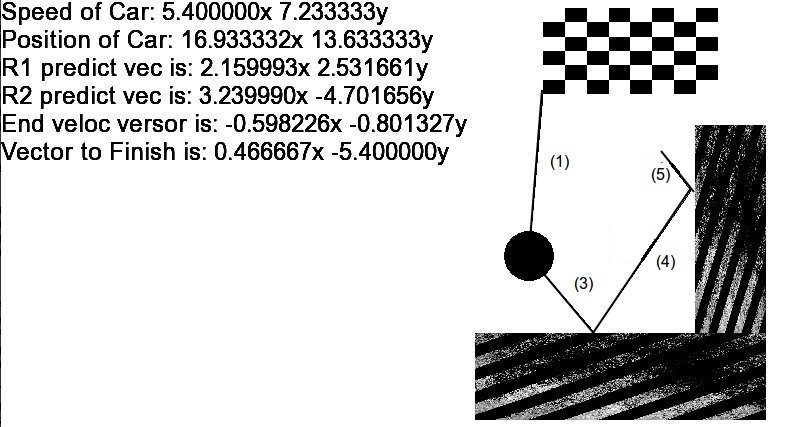
\includegraphics[width=\textwidth]{rys1.jpg}
	\caption{Wizualizacja informacji przekazywanych do sieci neuronowej.}
\end{figure}

\newpage

\section{Przeprowadzone testy.}
\subsection{Nauka trafiania do obszaru końcowego bez przeszkód.}

\indent Na torze został naniesiony jeden obszar końcowy i nie umieszczono na nim żadnych barier. Kolejno wprowadzano punkty danych do uczenia się sieci. Z obserwacji wynikły następujące wnioski:

\begin{enumerate}
		\item Wprowadzenie danych obiektu o położeniu i prędkościach tak jak na rysunku 2., wraz z decyzjami, wystarczyło by sterowany obiekt krążył w okolicach obszaru końcowego. W ciągu paru sekund obiekt docierał do obszaru końcowego.
			\item Zmniejszenie obszaru końcowego powodowało zatrzymanie się obiektu w okolicach samego obszaru końcowego - po wprowadzeniu paru dodatkowych punktów danych wraz z decyzjami dla procesu uczenia się obiekt  sterowany praktycznie z każdego miejsca toru odnajdywał prostą drogę do celu.
				\item Po zmianie położenia obszaru końcowego sieć nie potrafiła go odnaleźć. Jednak wprowadzenie takiej sekwencji  danych uczących jak pokazano na rysunku 2.  w dwóch kolejnych położeniach obszaru końcowego eliminowało tą zależność.
					\item Po uwzględnieniu powyższych uwag można stwierdzić, że zastosowana struktura sieci bez problemu radzi z sobie z postawionym problemem.
					\item Sygnały wejściowe redukowały się (ze względu na brak barier) do informacji o położeniu względnym obiektu oraz jego prędkości, co w zupełności wystarczyło.
\end{enumerate}

\begin{figure}
	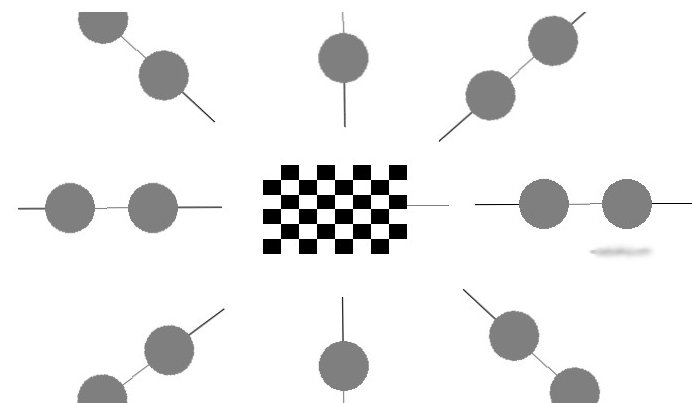
\includegraphics[width=\textwidth]{rys2.jpg}
	\caption{Położenia i prędkości wprowadzanych punktów dla nauki lokalizowania obszaru końcowego bez barier.}
\end{figure}

\newpage

\indent Nauka trafiania do obszaru z ominięciem przeszkody.

\indent Nauka trafiania do obszaru końcowego z wykorzystaniem odbicia się od przeszkody.

\end{document}
